\documentclass{article}
\usepackage{enumerate}
\usepackage{amssymb}
\usepackage{relsize}
\usepackage{fullpage}
\usepackage{amsmath}
\usepackage{tikz}
\usetikzlibrary{arrows, automata}
\usepackage[english]{babel}
\usepackage[utf8x]{inputenc}
\usepackage{enumitem}
\usepackage{mathtools}
\allowdisplaybreaks

\newcommand{\floor}[1]{\lfloor #1 \rfloor}
\newcommand{\ceil}[1]{\lceil #1 \rceil}
\newcommand{\Z}{\mathbb{Z}}
\newcommand{\R}{\mathbb{R}}
\newcommand{\N}{\mathbb{N}}
\newcommand{\fancyL}{\mathcal{L}}
\newcommand{\bigO}{\mathcal{O}}
\DeclareRobustCommand*\circled[1]{\tikz[baseline =(char.base)]{\node[shape=circle, draw, inner sep = 2pt] (char) {#1};}}


\title{CSC236 Problem Set 3}
\author{Jacob Nazarenko, James Currier, Mark Abdullah}
 
\begin{document}
\maketitle
\begin{enumerate}
	
	\item 
	a) (11)(0+01+011)*(01+011)\\\\
	b) ((1+00)(0+1)*(0*+10+11))+0+1+10+11+00\\
	
	
	
	\item
	 \text{ }\\
	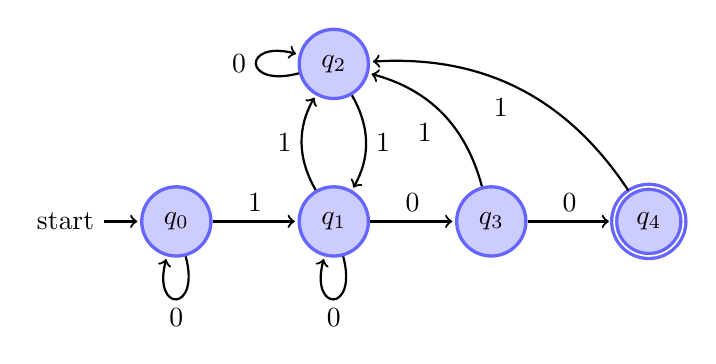
\begin{tikzpicture}[shorten >=1pt,thick,node distance=2cm,auto]
		\tikzstyle{every state}=[draw=blue!60,very thick,fill=blue!20]
		
		\node[state,initial] (q_0) {$q_0$};
		\node[state] (q_1) [right of=q_0] {$q_1$};
		\node[state] (q_2) [above of=q_1] {$q_2$};
		\node[state] (q_3) [right of=q_1] {$q_3$};
		\node[state, accepting] (q_4) [right of=q_3] {$q_4$};
		
		\path[->]
		(q_0)
		edge [loop below] node {0} ()
		edge node {1} (q_1)
		
		(q_1)
		edge [loop below] node {0} ()
		edge node {0} (q_3)
		edge [bend left] node {1} (q_2)
		
		(q_2)
		edge [loop left] node {0} ()
		edge [bend left]node {1} (q_1)
		
		(q_3)
		edge node {0} (q_4)
		edge [bend right] node {1} (q_2)
		
		(q_4)
		edge [bend right] node {1} (q_2);
		
		
	\end{tikzpicture}
	
	\item
	a)\\
	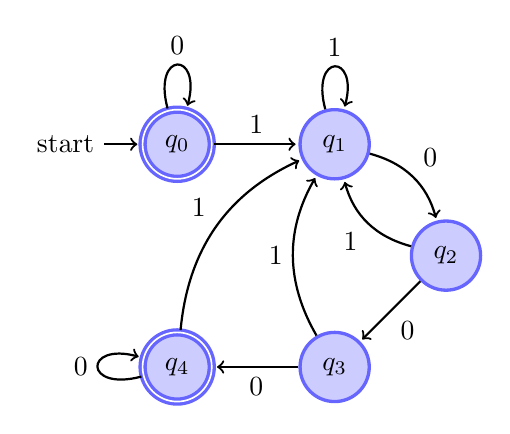
\begin{tikzpicture}[shorten >=1pt,thick,node distance=2cm,auto]
		\tikzstyle{every state}=[draw=blue!60,very thick,fill=blue!20]
		
		\node[state,initial,accepting] (q_0) {$q_0$};
		\node[state] (q_1) [right of=q_0] {$q_1$};
		\node[state](q_2) [below right of=q_1] {$q_2$};
		\node[state](q_3) [below left of=q_2] {$q_3$};
		\node[state,accepting](q_4) [left of=q_3] {$q_4$};
	
		\path[->] 	
		(q_0) 
		edge node {1} (q_1)
		edge [loop above] node {0} ()
		(q_1)
		edge [bend left] node {0} (q_2)
		edge [loop above] node {1} ()
		(q_2)
		edge node {0} (q_3)
		edge [bend left] node {1} (q_1)
		(q_3)
		edge node {0} (q_4)
		edge [bend left] node {1} (q_1)
		(q_4)
		edge [loop left] node {0} ()
		edge [bend left] node {1} (q_1);

	\end{tikzpicture} \\\\\\
	\[
	P(x):\ \ \  \delta^*(q_0, x)=  
	\begin{cases}
	q_0, & \text{if $x$ represents 0 (is all 0s)} \\
	q_1, & \text{if $x$ ends in a 1} \\
	q_2, & \text{if $x$ ends in a 1 followed by one 0} \\
	q_3, & \text{if $x$ ends in a 1 followed by two 0s} \\
	q_4, & \text{if $x$ ends in a 1 followed by three or more 0s}
	\end{cases}
	\] \\\\\\\\
	b)\\
	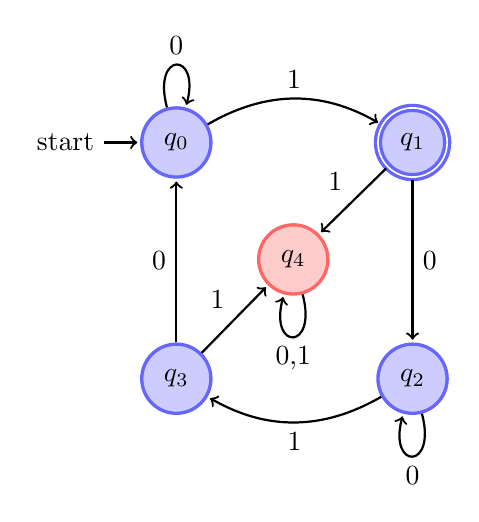
\begin{tikzpicture}[shorten >=1pt,thick,node distance=3cm,auto]
		\tikzstyle{every state}=[draw=blue!60,very thick,fill=blue!20]
		
		\node[state,initial] (q_0) {$q_0$};
		\node[state,accepting] (q_1) [right of=q_0] {$q_1$};
		\node[state] (q_2) [below of=q_1] {$q_2$};
		\node[state] (q_3) [left of=q_2] {$q_3$};
		\node[state,node distance=2.1cm,draw=red!60,fill=red!20] (q_4) [below right of=q_0] {$q_4$};
		
		
		\path[->] 	
		(q_0)
		edge [loop above] node {0} () 	
		edge [bend left]node {1} (q_1)
		(q_1)
		edge node{0} (q_2)
		edge [swap] node{1} (q_4)
		(q_2)
		edge [loop below] node{0} ()
		edge [bend left] node {1} (q_3)
		(q_3)
		edge node {0} (q_0)
		edge node{1} (q_4)
		(q_4)
		edge [loop below] node{0,1} ();
	
	\end{tikzpicture} \\\\\\
	\[
	P(x):\ \ \  \delta^*(q_0, x)=  
	\begin{cases}
	q_0, & \text{if $x$ has an even \# of 1s and ends with 0} \\
	q_1, & \text{if $x$ has an odd \# of 1s and ends with 1} \\
	q_2, & \text{if $x$ has an odd \# of 1s and ends with 0} \\
	q_3, & \text{if $x$ has an even \# of 1s and ends with 1}
	\end{cases}
	\] \\\\
	
	\item a) \\
	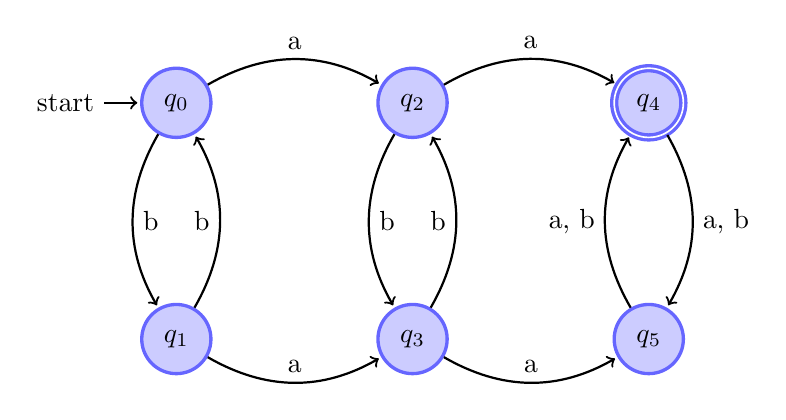
\begin{tikzpicture}[shorten >=1pt,thick,node distance=3cm,auto]
		\tikzstyle{every state}=[draw=blue!60,very thick,fill=blue!20]
		
		\node[state,initial] (q_0) {$q_0$};
		\node[state] (q_1) [below of=q_0] {$q_1$};
		\node[state] (q_2) [right of=q_0] {$q_2$};
		\node[state] (q_3) [right of=q_1] {$q_3$};
		\node[state, accepting] (q_4) [right of=q_2] {$q_4$};
		\node[state] (q_5) [below of = q_4] {$q_5$};
		
		
		\path[->] 	
		(q_0)
		edge [bend left] node {a} (q_2)
		edge [bend right] node {b} (q_1)
		
		(q_1)
		edge [bend right] node {a} (q_3)
		edge [bend right] node {b} (q_0)
		
		(q_2)
		edge [bend left] node {a} (q_4)
		edge [bend right] node {b} (q_3)
		
		(q_3)
		edge [bend right] node {a} (q_5)
		edge [bend right] node {b} (q_2)
		
		(q_4) edge [bend left] node {a, b} (q_5)
		
		(q_5) edge [bend left] node {a, b} (q_4);


\end{tikzpicture} \\\\\\
	\[
	P(x):\ \ \  \delta^*(q_0, x)=  
	\begin{cases}
	q_0, & \text{if $x$ has even length and zero a's} \\
	q_1, & \text{if $x$ has odd length and zero a's} \\
	q_2, & \text{if $x$ has odd length and one a} \\
	q_3, & \text{if $x$ has even length and one a} \\
	q_4, & \text{if $x$ has even length and two or more a's} \\
	q_5, & \text{if $x$ has odd length and two or more a's} \\
	\end{cases}
	\] \\
	
	b) Let  $\fancyL(D)$ represent the language accepted by the DFA above. We want to prove that $L = \fancyL(D)$ \\
	Let us begin by proving $P(x)$ holds $\forall x \in \sum^*$
	
	\textbf{Proof (by induction):}\\
	\textbf{Base case: $x = \epsilon$}\\
	 $$\delta^*(q_0, x) =  \delta^*(q_0, \epsilon) = q_0 \implies P(\epsilon)\ \text{holds}$$
	 
	\textbf{Inductive Step:}\\
	Let $x \in \sum^*$ and $m \in \sum$. Assume P(x) [IH].\\\\
	\textbf{Case 1}: Assume m = a\\
	
	\textbf{Case 1.1}: $x$ has even length and zero $a$'s. \\
	Then $xm$ has odd length and one $a$.\\
	By [IH]  $\delta^*(q_0, x) = q_0$\\
	By definition,
	\begin{align*}
	\delta^*(q_0, xm) &= \delta^*(\delta^*(q_0, x), m)\\
	&= \delta^*(q_0, m)\\
	&= \delta^*(q_0, a) \\
	&= q2
	\end{align*}
	Therefore $P(xm)$ holds. \\
	
	\textbf{Case 1.2}: $x$ has odd length and zero $a$'s. \\
	Then $xm$ has even length and one $a$.\\
	By [IH]  $\delta^*(q_0, x) = q_1$\\
	By definition,
	\begin{align*}
	\delta^*(q_0, xm) &= \delta^*(\delta^*(q_0, x), m)\\
	&= \delta^*(q_1, m)\\
	&= \delta^*(q_1, a) \\
	&= q3
	\end{align*}
	Therefore $P(xm)$ holds. \\
	
	\textbf{Case 1.3}: $x$ has odd length and one $a$'s. \\
	Then $xm$ has even length and two $a$.\\
	By [IH]  $\delta^*(q_0, x) = q_2$\\
	By definition,
	\begin{align*}
	\delta^*(q_0, xm) &= \delta^*(\delta^*(q_0, x), m)\\
	&= \delta^*(q_2, m)\\
	&= \delta^*(q_2, a) \\
	&= q4
	\end{align*}
	Therefore $P(xm)$ holds. \\
	
	\textbf{Case 1.4}: $x$ has even length and one $a$'s. \\
	Then $xm$ has odd length and two $a$.\\
	By [IH]  $\delta^*(q_0, x) = q_3$\\
	By definition,
	\begin{align*}
	\delta^*(q_0, xm) &= \delta^*(\delta^*(q_0, x), m)\\
	&= \delta^*(q_3, m)\\
	&= \delta^*(q_3, a) \\
	&= q5
	\end{align*}
	Therefore $P(xm)$ holds. \\
	
	\textbf{Case 1.5}: $x$ has even length and two or more $a$'s. \\
	Then $xm$ has odd length and greater then two $a$.\\
	By [IH]  $\delta^*(q_0, x) = q_4$\\
	By definition,
	\begin{align*}
	\delta^*(q_0, xm) &= \delta^*(\delta^*(q_0, x), m)\\
	&= \delta^*(q_4, m)\\
	&= \delta^*(q_4, a) \\
	&= q5
	\end{align*}
	Therefore $P(xm)$ holds. \\
	
	\textbf{Case 1.6}: $x$ has odd length and two or more $a$'s. \\
	Then $xm$ has even length and greater than two $a$'s.\\
	By [IH]  $\delta^*(q_0, x) = q_5$\\
	By definition,
	\begin{align*}
	\delta^*(q_0, xm) &= \delta^*(\delta^*(q_0, x), m)\\
	&= \delta^*(q_5, m)\\
	&= \delta^*(q_5, a) \\
	&= q4
	\end{align*}
	Therefore $P(xm)$ holds. \\	
	
	
	\textbf{Case 2}: Assume m = b\\
	
	\textbf{Case 2.1}: $x$ has even length and zero $a$'s. \\
	Then $xm$ has odd length and zero $a$.\\
	By [IH]  $\delta^*(q_0, x) = q_0$\\
	By definition,
	\begin{align*}
	\delta^*(q_0, xm) &= \delta^*(\delta^*(q_0, x), m)\\
	&= \delta^*(q_0, m)\\
	&= \delta^*(q_0, b) \\
	&= q1
	\end{align*}
	Therefore $P(xm)$ holds. \\
	
	\textbf{Case 2.2}: $x$ has odd length and zero $a$'s. \\
	Then $xm$ has even length and zero $a$.\\
	By [IH]  $\delta^*(q_0, x) = q_1$\\
	By definition,
	\begin{align*}
	\delta^*(q_0, xm) &= \delta^*(\delta^*(q_0, x), m)\\
	&= \delta^*(q_1, m)\\
	&= \delta^*(q_1, b) \\
	&= q0
	\end{align*}
	Therefore $P(xm)$ holds. \\
	
	\textbf{Case 2.3}: $x$ has odd length and one $a$'s. \\
	Then $xm$ has even length and one $a$.\\
	By [IH]  $\delta^*(q_0, x) = q_2$\\
	By definition,
	\begin{align*}
	\delta^*(q_0, xm) &= \delta^*(\delta^*(q_0, x), m)\\
	&= \delta^*(q_2, m)\\
	&= \delta^*(q_2, b) \\
	&= q3
	\end{align*}
	Therefore $P(xm)$ holds. \\
	
	\textbf{Case 2.4}: $x$ has even length and one $a$'s. \\
	Then $xm$ has odd length and one $a$.\\
	By [IH]  $\delta^*(q_0, x) = q_3$\\
	By definition,
	\begin{align*}
	\delta^*(q_0, xm) &= \delta^*(\delta^*(q_0, x), m)\\
	&= \delta^*(q_3, m)\\
	&= \delta^*(q_3, b) \\
	&= q2
	\end{align*}
	Therefore $P(xm)$ holds. \\
	
	\textbf{Case 2.5}: $x$ has even length and two or more $a$'s. \\
	Then $xm$ has odd length and two or more $a$.\\
	By [IH]  $\delta^*(q_0, x) = q_4$\\
	By definition,
	\begin{align*}
	\delta^*(q_0, xm) &= \delta^*(\delta^*(q_0, x), m)\\
	&= \delta^*(q_4, m)\\
	&= \delta^*(q_4, b) \\
	&= q5
	\end{align*}
	Therefore $P(xm)$ holds. \\
	
	\textbf{Case 2.6}: $x$ has odd length and two or more $a$'s. \\
	Then $xm$ has even length and two or more $a$.\\
	By [IH]  $\delta^*(q_0, x) = q_5$\\
	By definition,
	\begin{align*}
	\delta^*(q_0, xm) &= \delta^*(\delta^*(q_0, x), m)\\
	&= \delta^*(q_5, m)\\
	&= \delta^*(q_5, b) \\
	&= q4
	\end{align*}
	Therefore $P(xm)$ holds. \\
	
	We have now shown that $P(xm)$ holds in every case. \\
	In conclusion, by the principle of Structural Induction, $P(w)$ holds $\forall w \in \sum^*$.\\
	
	We will now show that, \\
	1) $L \subseteq \fancyL(D)$\\
	2) $\fancyL(D) \subseteq L$\\
	
	1) Let $w \in L$, Then $w$ has even length and at least two $a$'s.\\
	\begin{align*}
	P(w) \text{ holds} &\implies \delta^*(q_0, w) = q4 \text{\ \ \ (an accepting state)}\\
	&\implies w \in \fancyL(D)\\
	&\implies L \subseteq \fancyL(D)
	\end{align*}
	
	2) Let $w \in \fancyL(D)$\\
	\begin{align*}
	P(w) \text{ holds and }  \delta^*(q_0, w) = q4 &\implies w \text{ has even length and two or more $a$'s}\\
	&\implies w \in L\\
	&\implies \fancyL(D) \subseteq L
	\end{align*}
	
	Then $$\fancyL(D) \subseteq L \text{ and }  L \subseteq \fancyL(D) \implies  L = \fancyL(D)$$
	Therefore we have proven the language $L$ and the language accepted by the DFA are equal, and hence the DFA is correct. \null\hfill $\blacksquare$ \\
	
	
	\item a) \textbf{Proof (by Contradiction):}\\
	We want to prove that $L_1$ is not a regular language. \\
  	Assume for contradiction that $L_1$ is a regular language. Then we will use the pumping lemma, which tells us there exists a pumping length $p$. \\
  	Let $s = a^{3p}b^p$ be a string in $L_1$.\\
  	Then by the pumping lemma there exists strings $x,y,z$ that satisfy the following, 
  	\begin{enumerate}[label = \arabic*.]
  	\item  $s = xyz =  a^{3p}b^p$
  	\item $|y| \geq 1$
  	\item $|xy| \leq p$
  	\item $\forall i \in \N, xy^iz \in L_1$
  	\end{enumerate}
  	
  	By this we know the the only possibility for $y$ is $a^k$ for $1\leq k \leq p$, since $|xy|$ must be less than $p$, and we know the first $3p$ characters of $s$ are all $a$'s.\\
  	By number 4, $xy^2z = a^{3p + k}b^p \in L_1$, however this cannot be true since this does not satisfy the condition of the language $L_1$ as stated in the question.\\
  	Therefore we have reached a contradiction, and $L_1$ cannot be a regular language. \null\hfill $\blacksquare$ \\
  	
  	b) \textbf{Proof (by Contradiction):}\\
  	We want to prove $L_2$ is not a regular language. \\
  	Assume for contradiction that $L_2$ is a regular language. \\
  	
  	Define $L' = L_2 \cap a^*b^* = \{ a^n b^m | m,n \in \N, n \leq m\}$\\
  	
  	The only way there are no $c$'s in a string in $L_2$ is if $m = n$ such that $a^nb^mc^{m-n} = a^nb^mc^0 = a^nb^m$. Then the complement of $L_2$ intersected with $a^*b^*$ must be in the form as described by the set notation of $L'$. \\
  	
  	Since regular languages are closed under intersection, and we know $a^*b^*$ is regular as it is represented by a regular expression, we get that $L'$ must also be regular, under the assumption that $L_2$ is regular. However it was proven in tutorial 10, question 2, that the set represented by $L'$ is not regular. We have reached a contradiction! \\
  	
  	Therefore, $L'$ not regular $\implies L_2$ not regular. \\
  	
  	We have thereby proven $L_2$ is not a regular language. \null\hfill $\blacksquare$ \\
  
  
\end{enumerate}
\end{document}